\documentclass[output=paper]{LSP/langsci} 
\ChapterDOI{10.5281/zenodo.1090962}
\title{Cognitive effort and explicitation in translation tasks}
\author{Igor A. Lourenço da Silva\affiliation{Universidade Federal de Uberlandia}%
% \href{mailto:ials@ufu.br}{ials@ufu.br}, \href{mailto:ialsigor@gmail.com}{ialsigor@gmail.com}
\lastand Adriana Silvina Pagano\affiliation{Universidade Federal de Minas Gerais}
% \href{mailto:apagano@ufmg.br}{apagano@ufmg.br}
}

\abstract{Drawing on the framework of systemic-functional linguistics, this paper examines cognitive effort for meaning explicitation in translation tasks. Two hypotheses were formulated building on \citet{Steiner2001Intralingual, Steiner2001Translations} and \citet{TirkkonenCondit2005}: (1) literal translation, as a default translation procedure/strategy, minimises cognitive effort; and (2) explicitation of more implicit realisations in the source text requires more cognitive effort. To test these hypotheses, 16 Brazilians and 16 Germans, proportionally distributed as field specialists and professional translators, were asked to perform a translation task of one of two versions of an L2 (English) source text into their L1. Both source text versions construed analogous meanings, but they had either the most explicit or the most implicit variants of ten agnate realisation pairs (five of each in each version). The task was recorded using the key-logging program Translog 2006. From a process-oriented perspective, the key-logged data were analysed to determine the renditions per variant, number of micro-units per word, number of pauses per word, and drafting time per word. From a product-oriented perspective, subjects' renditions were analysed to investigate the impact of their choices on the explicitness and implicitness of the target texts. Overall, the results confirm the hypothesis that literal translation is a default procedure that requires less cognitive effort. As to the second hypothesis, more implicit variants in the source text do not necessarily require more cognitive effort than their less implicit variants.}

% Keywords: Translation process. Translation product. Cognitive effort. Literal translation. Explicitation. Default translation procedure.

\maketitle
\begin{document}

\section{Introduction}

Building on empirical-experimental research, \citet{TirkkonenCondit2005} hypothesises that `literal' translation, i.e., opting for wordings in the target text (TT) that are closely patterned upon the lexico-grammar of the source text (ST), is a default \isi{translation procedure}/strategy adopted by both experts and \isi{novices}. Assuming that similar lexico-grammatical patterns entail similar levels of explicitness in wordings \citet{Steiner2001Translations} and that the human translator as a `cognitive miser' \citep{Fiske1984} resorts to \isi{explicitation} as a complex strategy for TT production when problem solving is demanded, \isi{literal translation}, as a default procedure, is expected to minimise \isi{cognitive effort}. According to Tirkkonen-Condit, a monitoring process called `\isi{monitor}', usually better developed in experts, enables translators to recognise instances in the ST that constitute translation problems unlikely to be solved through a \isi{literal translation} strategy.

If \isi{literal translation} is a default procedure in translation and it involves similar lexico-grammatical patterns, translated texts would be expected to evidence a good deal of shared level of explicitness with their source counterparts. However, corpus-based research has pointed to translated texts as being more explicit %
%see also work by Mona Baker and Maeve Olohan on the optional {\textquotedbl}that{\textquotedbl} in English translations compared to non{}-translated English
%
%
%This study is referred to further down in the article
%
\citep{Olohan2000, Steiner2001Intralingual, Steiner2001Translations}. Explicitation has been reported as a phenomenon partially accounted for by typological differences between source and target languages as well as differences in the source and target contexts of culture and situation. In addition, a third source of \isi{explicitation} has been claimed to be translators' understanding of the ST and its role in TT production \citep{Steiner2001Intralingual, Steiner2001Translations}. 

Drawing on insights of both empirical-experimental research and corpus-based research, this paper reports on a process and product-oriented investigation of \isi{explicitation} with a view to testing two hypotheses, namely: 

\begin{itemize}
\item \isi{literal translation}, as a default \isi{translation procedure}, minimises \isi{cognitive effort}; 
\item translating more implicit realisations in the ST requires \isi{explicitation} on the translator's part, which entails an effortful \isi{translation procedure}.
\end{itemize}

To test these hypotheses, 16 Brazilians and 16 Germans, proportionally distributed as field specialists and professional translators, were asked to perform a task of translation of one of two versions of an L2 (English) ST into their L1. Both versions construed analogous meanings, but they had either the most explicited or the most implicited variants of ten agnate realisation pairs (five of each in each version). The task was recorded using the key-logging program Translog 2006. To operationalise an investigation of `literal' translation and \isi{explicitation}, we relied on the notions of `grammatical \isi{metaphor}' and `de-meta\-phor\-i\-sa\-tion' as expounded in the Literature Review.

This paper is made up of five sections including this Introduction. The Literature Review section provides the framework that was used to support this study. The Methodology section describes materials and methods for data collection and analysis. The Results and Discussion section focuses on the analysis of key-logging data. The Final Remarks section summarises our findings and points out future research avenues.

\section{Literature review} 

According to \citet{TirkkonenCondit2005}, translators tend to adopt the default, less effortful strategy of providing renditions patterned upon the ST -- i.e., `literal' translations. However, as translators move up in the novice-expert cline, they increasingly develop a monitoring mechanism (Monitor) that enables them to abandon such a strategy when they recognise ST patterns that require more careful attention due to \isi{target language} constraints. 

The tendency to use `literal' translation can be seen in \isi{translation process} data, as \citet{TirkkonenCondit2005} argues, when first renditions are examined. These tend to be reached by \isi{novices} and experts through automatism and are subsequently revised, as shown by interim renditions, when the Monitor mechanism is activated, usually in the case of more expert performance. In a \citeyear{TirkkonenCondit2006} study, Tirkkonen-Condit, along with Mäkisalo and Immonen, investigated the changes implemented by professional translators in the \isi{drafting phase} and found out that 40\% of the revisions were triggered by the need for adjusting instances that had previously been literally translated.

Automatism is ascribed by Tirkkonen-Condit to solutions patterned on the \isi{source language} lexico-grammar and to translation at ranks lower than the clause (e.g., word). Working at higher ranks and dealing with rearrangement of meanings differently construed in the ST and TT are assumed to be instances of the Monitor mechanism at work \citep[409]{TirkkonenCondit2005} and can be deemed as instances of effortful TT production. One such example is \isi{explicitation}, a phenomenon that has been investigated in studies of both translated text (e.g. \citealt{BlumKulka1986, Klaudy1998}) and \isi{translation process} (e.g., \citealt{Seguinot1988, Englund1993, Englund2005, Alves2011Modeling, Carl2012Inside, Schaeffer2013The, Carl2014Word, Halverson2015}).

Explicitation, as explained by \citet{Hansen2007}, is a process or a relationship between intralingual variants and/or translationally related texts. 

We assume \isi{explicitation} if a translation (or, language-internally, one text in a pair of register-related texts) realizes meaning (not only ideational, but also interpersonal and textual) more explicitly than its source text -- more precisely, meanings not realized in the less explicit source variant but implicitly present in a theoretically motivated sense. The resulting text is more explicit than its counterpart \citep[243]{Hansen2007}.

\citet[243]{Hansen2007} point out, and we follow suit, that their definition deliberately excludes the indefinite number of possibilities through which meaning can simply be added to some text/discourse, without being in any motivated sense implicit in the source variant. In their approach, \isi{explicitation} is characterised by a comparative measurement of explicitness as a property of encoding, not as a property of the communicative act as such. In other words, explicitness is a property of lexico-grammatical or cohesive structures and configurations, and \isi{explicitation} is the result of a process taking place in rewording tasks such as paraphrasing and translation.

From the very first process-oriented studies \citep{Seguinot1988, Englund1993}, \isi{explicitation} has been reported to be a phenomenon partially accounted for by typological differences between source and target languages as well as differences in the source and target contexts of culture and situation. However, \citet{Steiner2001Intralingual, Steiner2001Translations}, building on the notion of \isi{explicitation} as a translation universal \citep{Baker1995, Baker1996} and further developing it as a property of translated texts empirically observable in corpora, has posited a model in which he adds a third factor that may account for \isi{explicitation}, namely understanding on the part of the translator%
%here, also Mona \citet{Baker1996} should be mentioned since she set the ground for this with her description of \isi{explicitation} as translation universal
%
%
%done
%
. 

Steiner models understanding as an operation of de-meta\-phor\-i\-sa\-tion. A key concept to this is \textit{grammatical metaphor} as conceived of by systemic functional linguistics (SFL, \citealt{Halliday1999, Halliday2004}) and defined as ``the phenomenon whereby a set of agnate (related) forms is present in the language having different mappings between the semantic and the grammatical categories'' \citep[7]{Halliday1999}. \figref{silva-pagano:fig:1}, elaborated with variants of a sentence used in our experiment, displays four agnate forms with different levels of grammatical \isi{metaphoricity} in a cline from less metaphorical, and hence more congruent, to more metaphorical and less congruent.

\begin{figure}
\centering
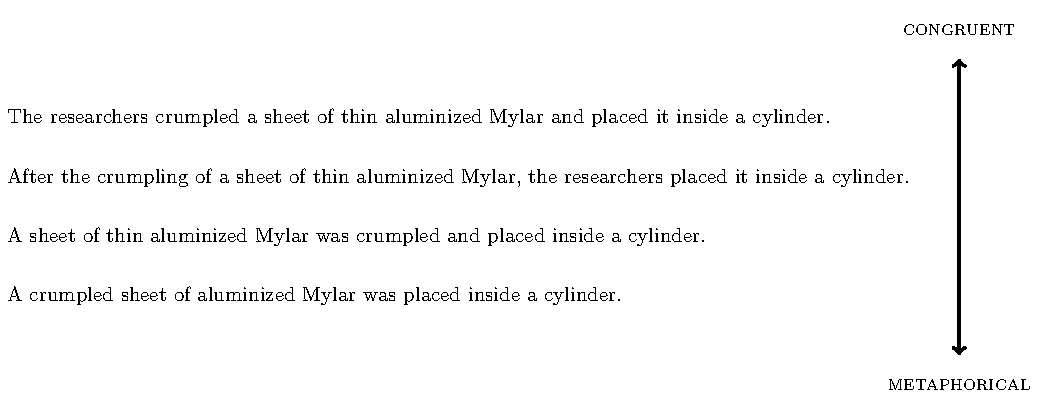
\includegraphics[width=\textwidth]{figures/silva-pagano/fig1.pdf} % recreated in tikz
\caption{Different levels of grammatical metaphoricity}
\label{silva-pagano:fig:1}
\end{figure}

As can be seen, congruency and \isi{metaphoricity} are a matter of level and may be identified through comparison of different agnate wordings. On the one hand, the more congruent wordings provide explicit agency (i.e., the researchers are the agents of the processes `to crumple' and `to place') and explicit causal and temporal relations (i.e., the researchers first crumpled the sheet of Mylar and then placed it inside a cylinder). On the other hand, the more metaphorical a wording, the more implicit and the more densely packed the meaning construed with increasing numbers of nominal forms and decreasing agency.

According to Steiner, understanding in translation involves mapping ST units onto their congruent meanings. This implies de-metaphorising and making meanings more explicit. As a result, due to typological features, registerial differences or understanding processes (also influenced by fatigue), the wordings produced in the TT may end up being less metaphorical than those in the ST. 

Within the discipline of translation studies, systematic differences in the\linebreak amount of explicated information between original and translated texts have been approached from different perspectives and theoretical standpoints through the concepts of \isi{implicitation} and \isi{explicitation} (see \citealt{Vinay1958Engl, BlumKulka1986, Seguinot1988, Klaudy1998, Olohan2000}, among others). In particular, \citet{Englund2005} is one of the few process studies, which draws on think-aloud protocols (TAPs) and key-logged data, to show how translators deal with \isi{explicitation}. Even though these concepts have proved very insightful and researchers have attempted to pin down their definitions, there remain many uncertainties as to how to measure what is a more explicit or implicit rendering of meaning. A more theoretically-informed approach to this issue draws on the aforementioned concept of grammatical \isi{metaphor}, which allows a more precise determination of what is explicit or implicit in a wording of meanings and where in the overall system of the language those meanings can be located.

To the best of our knowledge, process-oriented studies that have, to a greater or lesser extent, drawn on the notions of `grammatical \isi{metaphor}' and `de-meta\-phor\-i\-sa\-tion' are \citet{Hansen2003, Liparini2008, Liparini2010, daSilva2007, Pagano2010Traducao}. In her translation experiment with a \isi{professional translator} and a translation student working in the \ili{German}-English and \ili{French}-English language pair (both L2-L1), Hansen observed that (1) re-meta\-phor\-i\-sa\-tion (i.e.,~providing renditions with \isi{metaphoricity} levels analogous to that in the ST) was the most frequent strategy, and (2) de-meta\-phor\-i\-sa\-tion was more frequent than metaphorisation (e.g.,~increasing \isi{metaphoricity level} in the TT compared to the ST) when the subjects worked under no \isi{time pressure}. Similarly, in an experiment involving novice translators working in the English-\ili{Portuguese} language pair (2008) and in an experiment involving professional translators working in the both English-\ili{Portuguese} and \ili{German}-\ili{Portuguese} language pairs (2010), Liparini Campos also found more instances of metaphorisation in under no \isi{time pressure} condition. However, contrary to Hansen, she identified metaphorisation as the most frequent strategy also under \isi{time pressure} condition. Finally, \citet{daSilva2007} and \citet{Pagano2010Traducao} analysed the L1-L2 \isi{translation process} and product of a Brazilian Medicine field specialist and showed how he managed to render a highly grammatically metaphorical English-language text. They noticed that de-meta\-phor\-i\-sa\-tion instances were at play during the entire \isi{translation process} before the production of more metaphorical realisations in the target text.

\section{Methodology}

The data analysed in this paper were collected in an experimental study described in \citet{daSilva2012} and \citet{Alves2014Effortful}. A group of 8 \ili{German} and 8 Brazilian professional translators and another group of 8 \ili{German} and 8 Brazilian physicists were recruited to take part in an experiment in which they translated an English ST (L2 for all subjects) into \ili{German} or \ili{Brazilian Portuguese}, their respective L1. 

Physicists were recruited as participants in the experiment in the capacity of field specialists who ``perform translation tasks as part of their daily work, but neither have formal education in translation nor claim to be translators'' \citep[264]{Pagano2013}. Given their domain knowledge and discourse knowledge, field specialists in many countries are considered considered successful disciplinary writers, in both their L1 and L2 (mostly, English) even though their texts usually undergo through some \isi{editing} before reaching the publication stage \citep{Vasconcellos2007}, and given their domain knowledge and discourse knowledge \citep{Scardamalia1991}, and despite their lack of formal training and experience in translation, therefore they constitute, along with professional translators, a rich source of insights to understanding tap into processes involved in the understanding and production of highly metaphorical texts \citep{Pagano2010Text} as is the case of scientific texts \citep{Halliday2006}.

Subjects were instructed to carry out their task with no \isi{time pressure} and with the sole external support of a general reference dictionary in electronic format. Their translation processes were key-logged using Translog 2006. A translation brief drafted in the subjects' L1 was displayed on the computer screen prior to the subjects being allowed access to the ST (displayed on the top half of the screen). English-\ili{Portuguese} language data were collected at Universidade Federal de Minas Gerais in Brazil, while English-\ili{German} language data were collected at Universität des Saarlandes in Germany. 

Subjects were randomly assigned one of two versions (A or B) of an ST on the behaviour of crumpled balls, which was manipulated from an original publication of a popular science magazine. Both versions construed analogous meanings, but they had either the most explicit or the most implicit variants of ten agnate realisation pairs (five of each in each version). For each of these variants we investigated the number of renditions (interim and final solutions) and the \isi{implicitation} levels of the first and last renditions, as well as their related number of micro-units (see definition below) per word, number of \isi{pauses} per word in intervals of 2.4 seconds (see \citealt{Jakobsen2005Instances} and below) or longer, and drafting (see \citealt{Jakobsen2002Translation} and below) time per word. The analysis focused exclusively on the sentence parts that varied, and most variables were computed per word to assure comparability across ST wordings and TT renditions. \figref{silva-pagano:fig:2} illustrates segmentation as carried out for the purposes of identifying variables in the key-logged data.


\begin{figure}
\raggedright
\textbf{\textit{Drafting}}
\begin{tabularx}{\textwidth}{l X}
\textbf{M1} & \wdpause \wdpause \wdpause \wdpause poruq \wdbackspace \wdbackspace que \wdblank \\
\textbf{M2} & \wdpause uma \wdblank bola \wdblank  \\
\textbf{M3} & \wdpause \wdpause [Ctrl\wdcursor][Ctrl\wdcursor]\wddelete \wddelete \wddelete a \\
\textbf{M4} & \wdpause \wdpause \wdtab amassada \wdblank se \wdblank compot \wdbackspace rta \wdblank \\
\textbf{M5} & \wdpause \wdpause \wdpause \wdpause \wdpause \wdpause \wdpause \wdpause \wdpause [\wdmouse][\wdmouse] como \wdblank \wdbackspace \wdbackspace \wdbackspace \wdbackspace \wdbackspace porque \wdblank \wddelete \wddown  \\
\textbf{M6} & \wdpause \wdpause \wdpause \wdpause \wdpause \wdpause \wdpause \wdpause \wdpause \wdpause \wdpause [\wdmouse][\wdmouse][\wdmouse]\\
\textbf{M7} & \wdpause \wdpause \wdpause \wdpause \wdpause \wdpause \wdpause \wdpause [\wdmouse][\wdmouse]\wdpause \wdpause  \\
\textbf{M8} & \wddown da \wdblank maneira \wdblank \\
\textbf{M9} & \wdpause \wdbackspace \wdbackspace \wdbackspace \wdbackspace \wdbackspace \wdbackspace \wdbackspace \wdbackspace \wdbackspace \wdbackspace  \\
\textbf{M10}& \wdpause \wdpause \wdpause \wdpause \wdpause \wdpause [\wdmouse] a \wdblank sua \wdblank maneira \wdblank  \\
\textbf{M11}& \wdpause \wdpause \wdpause \wdpause \wdpause \wdpause \wdpause [\wdmouse]de \wdblank uma \wdblank maneira \wdblank particular \wdblank 
\end{tabularx}

\vspace{1em}
\textbf{\textit{Revision}}
\begin{tabularx}{\textwidth}{l X}
\textbf{M12} & \wdpause \wdpause \wdpause \wdpause \wdpause \wdpause \wdpause \wdpause \wdpause \wdpause \wdpause \wdpause \wdpause [\wdmouse][\wdmouse] peculiar \wdblank \wdbackspace \wdpause \wdpause 
\end{tabularx}


\vspace{1em}
\footnotesize\centering\textit{Note}: \wdpause = pause intervals of 2.4 seconds, \wdblank  = blank spaces, \wdcursor = cursor left, \wdbackspace  = backspace, \wddelete  = delete, \wdtab = tab key

\caption{Portuguese language rendition by BP1 for ``why the crumpled ball behaves the way it does''}
\label{silva-pagano:fig:2}
\end{figure}

\figref{silva-pagano:fig:2} shows a total of 12 micro-units -- 11 in the \isi{drafting phase}, and 1 in the \isi{revision} phase. According to \citet{Jakobsen2002Translation}, the \isi{drafting phase} starts when the subject types the first character and ends when s/he types, for the first time, the last character that concludes a preliminary first version of the TT, while the \isi{revision} phase starts immediately after the \isi{drafting phase} and ends when the subject completes the task. In this study, each rendition was assigned to either the drafting or the \isi{revision} phase, and only those in the \isi{drafting phase} had their duration computed.


Following \citet[107]{Alves2011On}, micro-units were observed in ``the flow of continuous TT production, which may incorporate the continuous reading of ST and TT segments, separated by \isi{pauses} during the \isi{translation process}''. In \figref{silva-pagano:fig:2}, the \isi{pauses} are represented by \wdpause and their duration is 2.4 seconds, a threshold determined by \citet{Jakobsen2005Instances}. 

  
First interim renditions were mapped and a new rendition was mapped onto it every time the subjects' keystrokes showed indications of recursiveness, such as deletion, backspacing, and mouse clicks, that were related to attempts at construing or \isi{revising} meaningful forms. The mapping concluded when subjects arrived at a final rendition in the TT. In \figref{silva-pagano:fig:2}, for instance, the \isi{first rendition} is \textit{``porque uma bola} [why a ball]'' (corresponding to micro-units M1 and M2), and the second rendition is \textit{``porque a bola} [why the ball]'' (micro-unit M3), since replacing the indefinite article \textit{``uma}'' with the definite article \textit{``a}'' was considered a meaningful change. Different renditions could also be found within the same micro-unit as in M5, in which the subject first replaced \textit{``porque} [why]'' (rendered in M1) with \textit{``como} [how]'', and then rendered back \textit{``porque}''. Notice that non-meaningful changes, such as correcting typos (as in M1: \textit{``poruq}'' instead of \textit{``porqu[e]}''), were not identified as new renditions. 

  
Each rendition had its grammatical \isi{metaphoricity level} determined. The met\-a\-phor\-icity level of the \isi{first rendition} was compared to that in the ST, and the \isi{metaphoricity level} of the last rendition was compared to that in the ST and the \isi{first rendition}.\footnote{This method ignored changes in interim renditions when the final solution was arrived at the third or further rendition (e.g., instances that first had the same level of \isi{metaphoricity}, were then modified in the interim version and switched back again in the final version). This is a trade-off we had to make to avoid \isi{noise} in the data: as \citet{Halliday1999, Steiner2001Intralingual, Steiner2001Translations} predict, de-meta\-phor\-i\-sa\-tion and metaphorisation may be necessary at a given point of a text in order to make it in all more implicit or more explicit. Despite this trade-off, we believe this method ensured the internal validity of our experiment, since we worked with a tendency of `literal' translation in the \isi{first rendition} (assuming it as a default procedure) and had the full \isi{metaphoricity level} in the final rendition.} Instances of `literal' translation were identified when the \isi{metaphoricity} levels tended to be analogous to that in the ST, instances of \isi{explicitation} were ascribed to reduced \isi{metaphoricity} levels, i.e. de-meta\-phor\-i\-sa\-tion. Implicitation was considered the opposite of \isi{explicitation} and ascribed to instances of increased \isi{metaphoricity} levels. 

  
Descriptive statistics (mean, standard deviation, and absolute and relative numbers) was used to explore the data. For some of the variables, we ran, whenever possible, non-parametric tests, namely Mann-Whitney U test or Fisher's exact test, using SPSS v. 17.0. The significance level was set at p<0.05. The tests were aimed at comparing ST versions (A and B), subjects' nationality (as a proxy for language pair), profile (translators/field specialists), \isi{metaphoricity level} of the \isi{first rendition} compared to that of the ST (analogous or non-analogous as proxies for `literal' translation and \isi{explicitation}/\isi{implicitation}, respectively), and \isi{metaphoricity level} of the final rendition compared to that of the ST (analogous, higher or lower as proxies for `literal' translation, \isi{implicitation} and \isi{explicitation}, respectively) and that of the \isi{first rendition} (analogous or non-analogous). 

  
Since first and interim renditions are on-going solutions, distinguishing (or rather predicting) de-meta\-phor\-i\-sa\-tion or metaphorisation (which fairly depends on further choices within a sentence) was not possible to all variants, and therefore the analysis was restricted to determining analogous or non-analogous renditions. Metaphorisation at a certain point may be followed by de-meta\-phor\-i\-sa\-tion further in the sentence, and vice-versa. 

  
In other words, this method ignored changes in interim renditions when the final solution was arrived at the third or further rendition (e.g., instances that first had the same level of \isi{metaphoricity}, were then modified in the interim version and switched back again in the final version). This is a trade-off we had to make to avoid \isi{noise} in the data: as \citet{Halliday1999, Steiner2001Intralingual, Steiner2001Translations} predict, de-meta\-phor\-i\-sa\-tion and metaphorisation may be necessary at a given point of a text in order to make it in all more implicit or more explicit. Despite this trade-off, we believe this method ensured the internal validity of our experiment, since we worked with a tendency of `literal' translation in the \isi{first rendition} (assuming it as a default procedure) and had the full \isi{metaphoricity level} in the final rendition.

\begin{itemize}
\item \isi{literal translation}, as a default \isi{translation procedure}, minimises \isi{cognitive effort}; 
\item translating more implicit realisations in the ST requires \isi{explicitation} on the translator's part, which entails an effortful \isi{translation procedure}.
\end{itemize}

Hypothesis (1) was expected to be confirmed through (1.1) a greater number of final solutions that were arrived at in the \isi{first rendition} tendency to keep the \isi{metaphoricity level} of the ST in both first and final renditions and (1.2) higher values for measures number of renditions, \isi{pauses} per word, drafting duration per word and micro-units per words in the production of non-analogous renditions. Hypothesis (2) would be confirmed through higher values for measures number of renditions, \isi{pauses} per word, drafting duration per word and micro-units per words in the translation of more metaphorical variants. 


Analyses for ST version (A or B), subject profile (\isi{professional translator} or field specialist) and subject nationality (Brazilian or \ili{German}) were expected to provide further insight into the matter. More specifically, we tested if those independent variables could (also) have an impact on the results.

\section{Results and discussion}

\tabref{silva-pagano:tab:1} shows the number of renditions till a final solution was arrived at by the two groups of subjects for the variants in each ST version used in the experiment. 

\begin{table}
\footnotesize
\centering
\begin{tabularx}{\textwidth}{X r r r r r r r r}
\lsptoprule
\multirow{3}{*}{Final solution arrived  at in the ...}  & \multicolumn{4}{c}{Version A variants} & \multicolumn{4}{c}{Version B variants}\\
\cmidrule(lr){2-5} \cmidrule(lr){6-9}                               
& \multicolumn{2}{c}{Brazilians} & \multicolumn{2}{c}{Germans} & \multicolumn{2}{c}{Brazilians} & \multicolumn{2}{c}{Germans}\\
\cmidrule(lr){2-3} \cmidrule(lr){4-5} \cmidrule(lr){6-7} \cmidrule(lr){8-9}
& \ccalign{n} & \ccalign{\%} & \ccalign{n} & \ccalign{\%}  & \ccalign{n} & \ccalign{\%} & \ccalign{n} & \ccalign{\%}    \\
\midrule
 ... \isi{first rendition}            & 44    & 55.00     & 33    & 41.25     & 44    & 55.00     & 32    & 40.00 \\
 ... second rendition           & 15    & 18.75     & 24    & 30.00     & 23    & 28.75     & 18    & 22.50 \\
 ... third rendition            & 6     & 7.50      & 12    & 15.00     & 8     & 10.00     & 16    & 20.00 \\
 ... fourth rendition           & 8     & 10.00     & 4     & 5.00      & 3     & 3.75      & 7     & 8.75 \\
 ... fifth rendition or further & 7     & 8.75      & 7     & 8.75      & 2     & 2.50      & 7     & 8.75 \\
\lspbottomrule
\end{tabularx}
\caption{Absolute and relative numbers of final solutions arrived at in the nth rendition per text version and subject nationality}
\label{silva-pagano:tab:1}
\end{table}

The \isi{first rendition} was frequently the final solution in the experiment with this occurring in 55\% of the renditions for variants in both versions A and B among the Brazilians and at least 40\% of the renditions among the Germans. Mann-Whitney U test pointed to no significant differences between versions A and B (p=0.235 among Brazilians; p=0.253 among Germans), but to significant differences between different nationalities (p=0.004). This may be interpreted as evidence of a tendency for the final solution to be the \isi{first rendition} in both nationality groups, though the Brazilians tended to resort to such a strategy even more often. Since extending the final solution to the fourth or further rendition seemed to be rarer among the subjects, this is a potential threshold to be used in further studies as indicative of additional \isi{cognitive effort} to produce the translated text.

\tabref{silva-pagano:tab:2} further explores general data in \tabref{silva-pagano:tab:1} to provide the results for the nth renditions and final solutions per subject nationality, subject profile, and \isi{metaphoricity level} of the variants in the ST.

\begin{table}
\footnotesize
\centering
\begin{tabularx}{\textwidth}{XXXXXXXXX}
\lsptoprule
\multirow{3}{*}{\parbox{4cm}{Final solution arrived \newline at in the ...}} & \multicolumn{4}{c}{Brazilians} & \multicolumn{4}{c}{Germans}\\
\cmidrule(lr){2-5} \cmidrule(lr){6-9}
                              & \multicolumn{2}{c}{Field Specialists} & \multicolumn{2}{c}{Translators} & \multicolumn{2}{c}{Field Specialists} & \multicolumn{2}{c}{Translators}\\
                                \cmidrule(lr){2-3} \cmidrule(lr){4-5} \cmidrule(lr){6-7} \cmidrule(lr){8-9}
 & \cralign{$\uparrow$} & \cralign{$\downarrow$} & \cralign{$\uparrow$} & \cralign{$\downarrow$} & \cralign{$\uparrow$} & \cralign{$\downarrow$} & \cralign{$\uparrow$} & \cralign{$\downarrow$}\\
\midrule
\ldots \isi{first rendition} & \cralign{22} & \cralign{19} & \cralign{26} & \cralign{21} & \cralign{20} & \cralign{19} & \cralign{16} & \cralign{10}\\
\ldots second rendition & \cralign{10} & \cralign{8} & \cralign{8} & \cralign{12} & \cralign{10} & \cralign{10} & \cralign{9} & \cralign{13}\\
\ldots third rendition & \cralign{2} & \cralign{3} & \cralign{1} & \cralign{3} & \cralign{7} & \cralign{6} & \cralign{7} & \cralign{8} \\
\ldots fifth rendition or further & \cralign{4} & \cralign{3} & \cralign{--} & \cralign{1} & \cralign{1} & \cralign{4} & \cralign{4} & \cralign{5}\\
\lspbottomrule
\end{tabularx}
\caption{Absolute and relative numbers of final solutions arrived at in the nth rendition per subject nationality, subject profile and metaphoricity level compared to that in the ST ($\uparrow$: high metaphoricity level variants; $\downarrow$: low metaphoricity level variants)}
\label{silva-pagano:tab:2}
\end{table}

In \tabref{silva-pagano:tab:2}, it is to be noted that instances of high \isi{metaphoricity} levels in the ST did not result in a higher number of renditions till the final solutions were arrived at than the instances of lower \isi{metaphoricity} levels. The number of final solutions arrived at in the first renditions was higher among the variants with higher \isi{metaphoricity} levels, regardless of profile and nationality. The difference, however, was not statistically significant.

\largerpage
\tabref{silva-pagano:tab:3} provides results on the \isi{metaphoricity level} of the first renditions compared to their respective ST variants. Results are split by nationality and ST version.

\begin{table}
\footnotesize
\centering
\begin{tabularx}{\textwidth}{XXXXXXXXX}
\lsptoprule
\multirow{3}{*}{\parbox{4cm}{Metaphoricity level of 1st rendition compared to that in the ST}} & \multicolumn{4}{c}{Brazilians} & \multicolumn{4}{c}{Germans}\\
\cmidrule(lr){2-5} \cmidrule(lr){6-9}
                                & \multicolumn{2}{c}{\parbox{1.25cm}{Version A variants}} & \multicolumn{2}{c}{\parbox{1.25cm}{Version B variants}} & \multicolumn{2}{c}{\parbox{1.25cm}{Version A variants}} & \multicolumn{2}{c}{\parbox{1.25cm}{Version B variants}}\\
                                \cmidrule(lr){2-3} \cmidrule(lr){4-5} \cmidrule(lr){6-7} \cmidrule(lr){8-9}
 & \ccalign{n} & \ccalign{\%} & \ccalign{n} & \ccalign{\%} & \ccalign{n} & \ccalign{\%} & \ccalign{n} & \ccalign{\%} \\
\midrule
Analogous       &  \cralign{57} &  \cralign{71.25} &  \cralign{67} &  \cralign{83.75} &  \cralign{58} &  \cralign{72.50} &  \cralign{65} & \cralign{81.25}\\
Non-analogous   &  \cralign{23} &  \cralign{28.75} &  \cralign{13} &  \cralign{16.25} &  \cralign{22} &  \cralign{27.50} &  \cralign{15} & \cralign{18.75}\\
Total           &  \cralign{80} &  \cralign{100.00}&  \cralign{80} &  \cralign{100.00}&  \cralign{80} &  \cralign{100.00}&  \cralign{80} & \cralign{100.00}\\
\lspbottomrule
\end{tabularx}
\caption{Absolute and relative numbers of first renditions with analogous or non-analogous metaphoricity levels compared to those in the ST per subject nationality and source text version variants}
\label{silva-pagano:tab:3}
\end{table}

As shown in \tabref{silva-pagano:tab:3}, the \isi{metaphoricity level} of the first solution tended to be analogous to that in the variants in both ST versions. That was so in 70\% of the sample. Fisher's exact test indicates that the difference of 12.5 percentage points between the ST versions is significant among the Brazilians (p=0.044), whereas the difference of 9.25 percentage points is not among the Germans (p=0.130).

The difference in the numbers of analogous and non-analogous renditions between the two ST versions may be ascribed to the Brazilians' performance in variants 5 and 8 and the Germans' performance in variant 8, because, as discussed in \citet{daSilva2012}, the metaphorical versions of these two variants required subjects to cope with complex translation problems related to typological and registerial differences between source and target languages. As such, they needed to be de-metaphorised, i.e., be made more explicit in the TT.

Excluding from the sample variants 5 and 8 from both text versions A and B (cf. \tabref{silva-pagano:tab:4}), the difference between the versions is no longer significance among both Brazilians (4.25 percentage points) and Germans (3.62 percentage points), with p=0.317 and p=0.413 among Brazilians and Germans, respectively. In other words, when highly influential typological and registerial differences are not at play, the first renditions do tend to have explicitness levels analogous to those in the ST wordings.

\begin{table}
\footnotesize
\centering
\begin{tabularx}{\textwidth}{XXXXXXXXX}
\lsptoprule
\multirow{3}{*}{\parbox{4cm}{Metaphoricity level of 1st rendition compared to that in the ST}} & \multicolumn{4}{c}{Brazilians} & \multicolumn{4}{c}{Germans}\\
\cmidrule(lr){2-5} \cmidrule(lr){6-9}
                                & \multicolumn{2}{c}{\parbox{1.25cm}{Version A variants}} & \multicolumn{2}{c}{\parbox{1.25cm}{Version B variants}} & \multicolumn{2}{c}{\parbox{1.25cm}{Version A variants}} & \multicolumn{2}{c}{\parbox{1.25cm}{Version B variants}}\\
                                \cmidrule(lr){2-3} \cmidrule(lr){4-5} \cmidrule(lr){6-7} \cmidrule(lr){8-9}
 & \ccalign{n} & \ccalign{\%} & \ccalign{n} & \ccalign{\%} & \ccalign{n} & \ccalign{\%} & \ccalign{n} & \ccalign{\%} \\
\midrule
Analogous       & \cralign{55}    &  \cralign{86.00}    & \cralign{52}    &  \cralign{81.75}    & \cralign{52}    &  \cralign{81.75}    & \cralign{50}    & \cralign{78.13} \\
Non-analogous   & \cralign{9}    &  \cralign{14.75}    & \cralign{12}    &  \cralign{18.25}    & \cralign{12}    &  \cralign{18.25}    & \cralign{14}    & \cralign{21.78} \\
Total           & \cralign{64}    &  \cralign{100.00}   & \cralign{64}    &  \cralign{100.00}   & \cralign{64}    &  \cralign{100.00}   & \cralign{64}    & \cralign{100.00}\\
\lspbottomrule
\end{tabularx}
\caption{Absolute and relative numbers of first renditions with analogous or non-analogous metaphoricity levels compared to those in the ST per subject nationality and text version (excluding variants 5 and 8 from both versions)}
\label{silva-pagano:tab:4}
\end{table}

\tabref{silva-pagano:tab:5} shows to what extent the tendency for first renditions to have met\-a\-phor\-i\-city levels analogous to those in the ST is also observed in the final solutions. The number of first renditions with \isi{metaphoricity} levels analogous to those in the ST is divided by the number of final renditions with \isi{metaphoricity} levels analogous to those in the ST.

\begin{table}
\footnotesize
\centering
\begin{tabularx}{\textwidth}{XXXXXXXX}
\lsptoprule 
\multicolumn{4}{c}{Brazilians} & \multicolumn{4}{c}{Germans}\\
\cmidrule(lr){1-4} \cmidrule(lr){5-8}
\multicolumn{2}{c}{Version A} & \multicolumn{2}{c}{Version B} & \multicolumn{2}{c}{Version A} & \multicolumn{2}{c}{Version B}\\
\cmidrule(lr){1-2} \cmidrule(lr){3-4} \cmidrule(lr){5-6} \cmidrule(lr){7-8}
\ccalign{n} & \ccalign{\%} & \ccalign{n} & \ccalign{\%} & \ccalign{n} & \ccalign{\%} & \ccalign{n} & \ccalign{\%} \\ \midrule
49/55 & 89.00 & 48/52 & 92.31 & 50/52 & 96.10 & 47/50 & 94.00\\
\lspbottomrule
\end{tabularx}
\caption{Tendency of keeping the metaphoricity level of the source text in both first and final renditions (excluding variants 5 and 8 from both versions)}
\label{silva-pagano:tab:5}
\end{table}

As shown in \tabref{silva-pagano:tab:5}, final solutions have \isi{metaphoricity} levels analogous to those in first renditions compared to the their ST counterparts. Such a tendency was of at least 89\% considering only analogous renditions and at least 73\% considering the lowest number (47) of analogous renditions and the total number of renditions (64 for Germans' translation of version B, excluding variants 5 and 8). 

Subtracting divisors from dividends in \tabref{silva-pagano:tab:5} we obtain the number of final renditions having \isi{metaphoricity} levels analogous to those in the ST though not necessarily so in first renditions. In total, that was the case of 15 (23\%) final renditions. This indicates that no more than 23\% of the total number of revisions made during a translation task has to do with \isi{metaphoricity} changes, the remaining 77\% being mostly related to changes in lexis rather than in grammar. 

\tabref{silva-pagano:tab:6} provides the absolute and relative number of final solutions comparing their \isi{metaphoricity} levels to those in the ST.

\begin{table}
\centering
\fittable{
\begin{tabular}{lcccccccc}
\lsptoprule
\multirow{3}{4cm}{Metaphoricity level of 1st rendition compared to that in the ST} & \multicolumn{4}{c}{Brazilians} & \multicolumn{4}{c}{Germans}\\
\cmidrule(lr){2-5} \cmidrule(lr){6-9}
& \multicolumn{2}{c}{$\uparrow$} & \multicolumn{2}{c}{$\downarrow$} & \multicolumn{2}{c}{$\uparrow$} & \multicolumn{2}{c}{$\downarrow$}\\
\cmidrule(lr){2-3} \cmidrule(lr){4-5} \cmidrule(lr){6-7} \cmidrule(lr){8-9}
& \ccalign{n} & \ccalign{\%} & \ccalign{n} & \ccalign{\%} & \ccalign{n} & \ccalign{\%} & \ccalign{n} & \ccalign{\%} \\ \midrule

Analogous & \cralign{49}& \cralign{76.56}  & \cralign{50} & \cralign{78.13}  & \cralign{50}  & \cralign{78.12}   & \cralign{51}  & \cralign{79.69}   \\
Higher  &  \cralign{8}  & \cralign{12.50}  & \cralign{12} & \cralign{18.75}  & \cralign{7}   & \cralign{10.94}   & \cralign{8}   & \cralign{12.50}   \\
Lower   &  \cralign{7}  & \cralign{10.94}  & \cralign{2}  & \cralign{3.12}   & \cralign{7}   & \cralign{10.94}   & \cralign{5}   & \cralign{7.81}    \\
Total   &  \cralign{64} & \cralign{100.00} & \cralign{64} & \cralign{100.00} & \cralign{64}  & \cralign{100.00}  & \cralign{64}  & \cralign{100.00}  \\
\lspbottomrule
\end{tabular}
}
\caption{Absolute and relative numbers of first renditions with analogous or non-analogous metaphoricity levels compared to those in the ST per subject nationality and metaphoricity level (excluding variants 5 and 8 from both versions; $\uparrow$: high metaphoricity level variants; $\downarrow$: low metaphoricity level variants)}
\label{silva-pagano:tab:6}
\end{table}

\largerpage
Confirming previous results provided above, \tabref{silva-pagano:tab:6} shows that at least 76.56\% instances of the variants were rendered with \isi{metaphoricity} levels analogous to those in the ST (i.e., `literal' translation). This seems to corroborate \citet{TirkkonenCondit2005} and to provide further food for thought regarding the concept, usefulness and potential role of `literal' translation forin both humans and machines translation (e.g. \citealt{Chesterman2011, Carl2014Word, Halverson2015}).

In addition, the results point to a slight tendency for decision making to involve metaphorisation (\isi{implicitation}, \isi{metaphoricity level} higher than that in the ST) rather than de-meta\-phor\-i\-sa\-tion (\isi{explicitation}, \isi{metaphoricity level} higher than that in the ST), namely 29 instances of metaphorisation (11 among physicists) vs. 27 instances of de-meta\-phor\-i\-sa\-tion (121 among translators), with no differences significantly ascribable to subject profile (Fisher's exact test: p>0.05). This seems to support da Silva's \citeyearpar{daSilva2007}, Liparini Campos's (\citeyear{Liparini2008}, \citeyear{Liparini2010}) and \citegen{Pagano2010Text} findings though run counter Hansen's \citeyearpar{Hansen2003} findings. 

In order to investigate whether `literal' translation is a cognitive effort-minim\-ising strategy and \isi{explicitation} and \isi{implicitation} require more \isi{cognitive effort}, a close look at \tabref{silva-pagano:tab:7} can be enlightening. \tabref{silva-pagano:tab:7} shows the means and standard deviations of four variables (number of renditions, \isi{pauses} per word, drafting time per word, and micro-units per word) per \isi{metaphoricity level} of the ST variant, ST version, subject profile, and subject nationality.
 
\begin{table}
\fittable{
\begin{tabular}{>{\raggedright}p{1.8cm} cccccccc}
\lsptoprule
\multirow{3}{2cm}{Variable} & 
\multicolumn{2}{c}{\parbox{2cm}{Metaphoricity level of the ST variant}} & 
\multicolumn{2}{c}{\parbox{3cm}{Source text version}} & 
\multicolumn{2}{c}{\parbox{3cm}{Subject profile}} &
\multicolumn{2}{c}{\parbox{3cm}{Subject nationality}}\\
\cmidrule(lr){2-3} \cmidrule(lr){4-5} \cmidrule(lr){6-7} \cmidrule(lr){8-9}
 & $\uparrow$ & $\downarrow$ & A & B & Translators & Field Specialists & Brazilians & Germans \\ \midrule
Number of renditions & 1.94 / 1.38 & 2.16 / 1.38 & 2.10 / 1.47 & 2.00 / 1.28 & 2.08 / 1.34 & 2.02 / 1.42 & 1.89 / 1.36 & 2.21/1.38\\
\tablevspace
Pauses per word & 1.59 / 2.08 & 1.53 / 1.56 & 1.62 / 2.20 & 1.51 / 1.39 & 1.27 / 1.48 & 1.86 / 2.10 & 1.43 / 2.11 & 1.69/1.51\\
\tablevspace
Drafting duration per word & 6.84 / 6.37 & 6.51 / 4.74 & 6.67 / 6.43 & 6.68 / 5.61 & 5.49 / 4.19 & 7.87 / 6.53 & 5.87 / 5.60 & 7.49/5.52\\
\tablevspace
\mbox{Micro-units} per word & 0.47 / 0.30 & 0.53 / 0.89 & 0.52 / 0.89 & 0.49 / 0.33 & 0.44 / 0.31 & 0.57 / 0.89 & 0.49 / 0.89 & 0.52/0.33\\
\lspbottomrule
\end{tabular}
}
\caption{Mean and standard deviation of cognitive effort measures per metaphoricity level of the source text variant, source text version, subject profile, and subject nationality}
\label{silva-pagano:tab:7}
\end{table}

\largerpage
The significance analysis of the data summarised in \tabref{silva-pagano:tab:7} points to no significant differences (p>0.05) for the variables when comparing within \isi{metaphoricity level} and within ST version. The result for ST version is reasonable, since versions A and B were carefully manipulated to be strongly comparable. However, the finding for \isi{metaphoricity level} somehow came as a surprise, since we expected that translating more metaphorical variants would be more effortful than translating less metaphorical variants. For two variables (number of renditions and micro-units per word), it was even more effortful to translate the less metaphorical variant. A potential explanation may be the fact that congruent sentences are not those with best readability \citep{Wolfer2015}, but this should be further investigated for the data in question.

As for the subject profile, the differences are significant (p<0.05) for all variables but number of renditions, i.e., translators were faster than the field specialists, since the translators had fewer \isi{pauses}, rendered words within a shorter interval, and needed less micro-units to accomplish the translation of each variant. These results are indicative of \isi{translation competence} \citep{Alves2007, PACTE2014}. 

As for subject nationality, the differences are significant (p<0.05) for all variables, i.e., the Brazilians were faster than the Germans when rendering the variants under scrutiny. These differences should be further explored, and may be ascribable to typological differences \citep{Steiner2001Intralingual, Steiner2001Translations}, different notions of translation \citep{Matthiessen2001, TirkkonenCondit2010} and/or differences in TT quality \citep{Alves2014Effortful}. 

A further step in our analysis was looking at the impact of the final solutions having or not \isi{metaphoricity} levels analogous to those in the ST variants. The results are displayed in \tabref{silva-pagano:tab:8}, where category `non-analogous' embraces both higher and lower \isi{metaphoricity} levels in the final renditions compared to those in the ST.

\begin{table}
\footnotesize
\begin{tabularx}{\textwidth}{lXX}
\lsptoprule
Variables per variant & Analogous (n = 247) & Non-analogous (n=73)\\
\midrule
Number of renditions & 1.95 / 1.32 & 2.40 / 1.50\\
Pauses per word & 1.46 / 1.54 & 1.93 / 2.58\\
Drafting duration per word & 6.35 / 4.57 & 7.80 / 8.14\\
Micro-units per word & 0.50 / 0.74 & 0.52 / 0.33\\
\lspbottomrule
\end{tabularx}
\caption{Mean and standard deviation of cognitive effort measures per metaphoricity level in the final rendition compared to that in the source text variant}
\label{silva-pagano:tab:8}
\end{table}

\largerpage
\tabref{silva-pagano:tab:8} seems to show that opting for more or less metaphorical wordings in the TT than in the ST has processual implications. For all variables, the means are higher when the \isi{metaphoricity level} in the TT is non-analogous to that in the ST. Bearing in mind that human beings are cognitive misers \citep{Fiske1984}, this result seems to corroborate that `literal' translation is a default, effort-minimising strategy, whereas alternative strategies are more cognitively effortful \citep{TirkkonenCondit2005}.

\section{Final remarks}

We set out this study aiming to test two hypotheses, namely:

\begin{itemize}
\item \isi{literal translation}, as a default \isi{translation procedure}, minimises \isi{cognitive effort}; 
\item translating more implicit realisations in the ST requires \isi{explicitation} on the translator's part, which entails an effortful \isi{translation procedure}.
\end{itemize}

Overall the results point to the independent variable (ST level of grammatical \isi{metaphoricity}) as having little or no impact on our dependent variables (i.e., number of renditions, total drafting time, number of \isi{pauses}, and number of micro-units). In other words, subjects do not seem to show more or less effort spent to translate a more or less metaphorical version of the ST. Our data suggest, however, that they do seem to invest more effort to change the level of grammatical \isi{metaphoricity} of their own previous solutions in cases of multiple interim renditions. 

In other words, the results confirm hypothesis (1) that the production of TT with lexico-grammatical realisations analogous to those in the ST is a default procedure and requires less \isi{cognitive effort}. Nevertheless, they do not confirm hypothesis (2) that more metaphorical variants in the ST require more \isi{cognitive effort} than the congruent variants. Returning to Tirkkonen-Condit's \citeyearpar{TirkkonenCondit2005} Monitor model, this additional effort may be ascribed to `literal' translation as a default procedure and to the activation of the \isi{monitor} mechanism as an effortful event. That seems to be much so that the variants that led to the highest occurrences of de-meta\-phor\-i\-sa\-tion were those having to do with constraints due to typological and registerial differences between source and target languages and revisions tended to involve changes in the lexical rather than in the grammatical pole.

De-meta\-phor\-i\-sa\-tion %
%please relate it to Baker's simplification
%
%
%Actually, simplification and de{}-metaphorisation are different processes
%
as an inherent property of translation has been probed in experimental studies of the \isi{translation process} by \citet{daSilva2007, daSilva2012, Alves2010, Alves2011Modeling, Alves2014Effortful, Alves2014Evidence}. All these studies have relied on the present data to account for different aspects of the \isi{translation process}, providing comparable analyses that complement each other. As stated in \citet{Alves2014Effortful, Alves2014Evidence}, however, more fine-grained data including analyses of the TT should be incorporated to cast further light on the role of \isi{explicitation} in translations tasks. Besides, the role played by subject profile and subject nationality (as a proxy for language pair) remains poorly explored and should be addressed more deeply. Yet, we believe that our effort to carry out such an extensive study will provide further insight on cognitive aspects of the \isi{translation process} and encourage collaborative work as the one involved in the experiment design and data collection.

\section*{Acknowledgements}

Research funded by the National Council for Scientific and Technological Development (CNPq) under grants No. 
307964/2011-6;
308652/2010-0;
308652/2010-0; 
305129/2013-9; and 
461054/2014-0; 
the State Funding Agency of Minas Gerais (FAPEMIG) under grants
SHA/PPM-00495-12; 
SHA/PPM-00087-12; 
PPM-00087-12; and
PPM-00289-14; 
the Coordination for the Improvement of Higher Education Personnel (CAPES) under grant Probral 292/08; and Universidade de Uberlandia under grant RECEM2014-0071.

\sloppy
\printbibliography[heading=subbibliography,notkeyword=this]
\end{document}

% \textbf{References}
% 
% Alves, F., Pagano, A.S. and da Silva, I.A.L. 2011. Modeling (Un)packing of Meaning in Translation: Insights from Effortful Text Production. In \textit{Proceedings of the 8th International NLPCS Workshop (Natural Language Processing and Cognitive Sciences). Special Theme: Human-Machine Interaction in Translation}, ed. by Bernadette Sharp, Michael Zock, Michael Carl, and Arnt L. Jakobsen. Copenhagen: Samfundslitterattur. p.153-162.
% 
% Alves, F., Pagano, A.S. and da Silva, I.A.L. 2014a. Effortful Text Production in Translation. A Study of Grammatical (De)metaphorization Drawing on Product and Process Data. \textit{Translation and Interpreting Studies} 9:1. p.25-51.
% 
% Alves, F., Pagano, A.S. and da Silva, I.A.L. 2014b. Evidence of De-metaphorization in Target Text Unfolding. In: Kunz, K., Teich, E., Hansen-Schirra, S., Neumann, S. and Daut, P. (eds.). \textit{Caught in the Middle?} Language Use and Translation. A Festschrift for Erich Steiner on the Occasion of his 60th Birthday. Saarbrücken: Universitätsverlag des Saarlandes. p.5-24.
% 
% Alves, F. and Vale, D. 2011. On drafting and \isi{revision} in translation: a corpus linguistics oriented analysis of \isi{translation process} data. \textit{Translation: Computation, Corpora, Cognition} 1:1. p.105-122.
% 
%  Alves, F.; Gonçalves, J. L. V. R. 2007 Modelling translator’s
% competence: relevance and expertise under scrutinity. In: Gambier, Y.;
% Schlesinger, M.; Stolze, R. (eds.). Translation Studies: doubts and
% directions. Selected papers from the IV Congress of the European
% Society for Translation Studies. Amsterdam: John Benjamins. p. 41-55.
% %
% Alves, Fabio et al., eds. 2010. New Approaches in Translation Process Research. Copenhagen: Samfundslitteratur Press.
%
%
%
% Baker, M. 1995. Corpora in Translation Studies: An Overview and Suggestions for Future Research. \textit{Target} 7:2. p.223-244 
% 
% Baker, M. 1996. Corpus-Based Translation Studies: The Challenges That Lie Ahead. In Somers, H. (ed.). \textit{Terminology, LSP and Translation Studies in Language Engineering. In Honour of Juan C. Sager}. Amsterdam/Philadelphia: John Benjamins. p.175-186 
% 
% Blum-Kulka, S. 1986. Shifts of Cohesion and Coherence in Translation. In House, J. and Blum-Kulka, S. (eds.). \textit{Interlingual and Intercultural Communication}, Tübingen: Narr. p.17--35.
% 
% Carl, M., and Barbara Dragsted. 2012. Inside the Monitor Model : Processes of Default and Challenged Translation Production. \textit{Translation: Computation, Corpora, Cognition} 2: 1. p.127-145. 
% 
% Carl, Michael,M. and Schaeffer, M. 2014. Word Transition Entropy as an Indicator for Expected Machine Translation Quality. In \textit{Proceedings of the Workshop on Automatic and Manual Metrics for Operational Translation Evaluation -- MTE 2014}, ed. by Keith J. Miller, Lucia Specia, Kim Harris, and Stacey Bailey. Paris: ELRA. p.45-50.
% 
% Chesterman, A. 2011. Reflections on the Literal Translation Hypothesis. In Alvstad, C., Hild, A. and Tiselius, E. \textit{Methods and Strategies of Process Research: Integrative Approaches in Translation Studies}. Amsterdam/Philadelphia: John Benjamins. p.23-35.
% 
% da Silva, I.A.L. 2007. Conhecimento Experto em Tradução: Aferição da Durabilidade de Tarefas Tradutórias Realizadas por Sujeitos Não-Tradutores em Condições Empírico-Experimentais. Unpublished PhD thesis, Universidade Federal de Minas Gerais.
% 
% da Silva, I.A.L. 2012. \textit{(Des)compactação de Significados e Esforço Cognitivo no Processo Tradutório: Um Estudo da Metáfora Gramatical na Construção do Texto Traduzido}. Unpublished PhD thesis, Universidade Federal de Minas Gerais.
% 
% Englund Dimitrova, B. 1993. Semantic Change in Translation. A Cognitive Perspective. In Gambier, Y. and Tommola, J. (eds). \textit{Translation and Knowledge}. Turku: Centre for Translation and Interpreting, University of Turku. p.285-296.
% 
% Englund-Dimitrova, B. 2005. \textit{Expertise and Explicitation in the Translation Process}. Amsterdam/Philadelphia: John Benjamins.
% 
% Fiske, S. T. and Taylor, Sh. E. 1984. Social cognition. Reading, MA:
%Addison-Wesley.
%
% Halliday, M.A.K. 2006. Some Grammatical Problems in Scientific English. In Webster, J. (ed.). \textit{The Language of Science.} London/New York: Continuum. p. 159-198. 
% 
% Halliday, M.A.K. and Matthiessen, C.I.M. 1999. \textit{Construing Experience through Meaning. A Language-Based Approach to Cognition}. London: Continuum.
% 
% Halliday, M.A.K. and Matthiessen, C.I.M. 2004. \textit{An Introduction to Functional Grammar}. 3. Ed. London: Arnold.
% 
% Halverson, S.L. 2015. \textit{Translation Spaces} 4:2. p.310-340.
% 
% Hansen, S. 2003. \textit{The Nature of Translated Text}. Saarbr\"{u}cken: Language Technology Lab.
% 
% Hansen-Schirra, S., Neumann, S. and Steiner, S. 2007. Cohesive Explicitness and Explicitation in an English-\ili{German} Translation Corpus. \textit{Languages in Contrast} 7:2. p.241-265.
% 
% Jakobsen, A.L. 2002. Translation Drafting by Professional Translators and by Translation Students. \textit{Traducción} \textit{\& Comunicación} 3. p.89-103.
% 
% Jakobsen, A.L. 2005. Instances of Peak Performance in Translation. \textit{Lebende Sprachen} 50:3. p.111-116.
% 
% Klaudy, K. 1998. Explicitation. In \textit{Encyclopedia of Translation Studies}, ed. by Baker, M. London: Routledge. p.80-85.
% 
% Liparini Campos, T. 2008. O Efeito da Pressão de Tempo na Realização de Tarefas de Tradução: Considerações sobre o Produto Tradutório. \textit{Revista da ABRALIN} 7: 2. p.223-241.
% 
% Liparini Campos, T. 2010. \textit{O Efeito do Uso de um Sistema de Memória de Tradução e da Pressão de Tempo no Processo Cognitivo de Tradutores Profissionais.} Unpublished PhD thesis, Universidade Federal de Minas Gerais.
% 
% Matthiessen, C. M. I. M. 2001. The Environments of Translation. In: Steiner, E. and Yallop, C. (eds.). \textit{Exploring Translation and Multilingual Text Production: Beyond Content}. Berlin: Mouton de Gruyter. 
% 
% Olohan, M. and Mona, B. 2000. Reporting \textit{That} in Translated English. Evidence for Subconscious Processes of Explicitation? \textit{Across Languages and Cultures} 1:2. p.141-158.
% 
% PACTE. 2014. First Results of PACTE Group's Experimental Research on Translation Competence Acquisition: The Acqusition of Declarative Knowledge of Translation. \textit{MonTI Special Issue -- Minding Translation}. p.85-115. 
% 
% Pagano, A.S. and da Silva, I.A.L. 2010a. Tradução e (Des)metaforização. 2010. In: Ghio, E. and Fernandez, M.D. (eds.). \textit{Estudios del Discurso en Español y Portugués desde una Perspectiva Sistémico-Funcional.} Santa Fe: Centro de Publicaciones de la Universidad Nacional Del Litoral. p.311-346.
% 
% Pagano, A.S. and da Silva, I.A.L. 2010b. Text Segmentation and Task Representation as Indicators of Translator's Performance: Insights from Translation Process Research. In \textit{Proceedings of the First International Conference on Translation and Interpretation}, ed. by Togtip Poonlarp. Bangkok: Chalermprakiat Centre of Translation and Interpretation. p.117-122.
% 
% Pagano, A.S., da Silva, I.A.L. and Alves, F. 2013. Tracing the Unfolding of Metaphorical Processes in Translation: Insights from an Experimental Exploratory Study. In \textit{Proceedings of the Maastricht Session of the 5th International Maastricht-Lódz Duo Colloquium on Translation and Meaning}, ed. by Marcel Thelen. Maastricht: Zuyd University -- Maastricht School of Translation and Interpreting. p.263-275.
% 
% Scardamalia, M. and Bereiter, C. 1991. Literate Expertise. In Ericsson, K.A. and Smith, J. (ed.). \textit{Toward a General Theory of Expertise}. Cambridge: CUP. p.172-194. 
% 
% Schaeffer, M. 2013. The Ideal Literal Translation Hypothesis: The Role of Shared Representations During Translation. Unpublished PhD Thesis, University of Leicester. 
% 
% Séguinot, C. 1988. Pragmatics and the Explicitation Hypothesis. \textit{TTR Traduction, Terminologie, Rédaction} 1:2. p.106-114.
% 
% Steiner, E. 2001a. Translations English-\ili{German}: Investigating the Relative Importance of Systemic Contrasts and of the Text Type {\textquotedbl}Translation{\textquotedbl}. \textit{SPRIKreports} 7. p.1-49.
% 
% Steiner, E. 2001b. Intralingual and Interlingual Versions of a Text: How Specific is the Notion of Translation. In: Steiner, E. and Yallop, C. (ed.). \textit{Exploring Translation and Multilingual Text Production}: Beyond Context. Berlin/New York: Mouton de Gruyter. p.161-190. 
% 
% Tirkkonen-Condit, S. 2005. The Monitor Model Revisited: Evidence from Process Research. \textit{Meta} 50:2. p.405-414.
% 
% Tirkkonen-Condit, S. 2010 Prototype Definition of Translation Revisited. In Lewandowska-Tomaszczyk, B. and Thelen, M. \textit{Meaning in Translation.} Frankfurt am Main: Peter Lang. p.217-230. 
% 
% Tirkkonen-Condit, S., Mäkisalo, J. and Immonen, S. 2006. The Translation Process: Interplay between Literal Rendering and a Search for Sense. \textit{Across Languages and Cultures: A~}\textit{Multidisciplinary Journal for Translation and Interpreting Studies} 9:1. p.1-15. 
% 
% Vasconcellos, S.M.R, Sorenson, M.M. and Leta. J. 2007. Scientist-Friendly Policies for Non-Native English-Speaking Authors: Timely and Welcome. \textit{Brazilian Journal of Medical and Biological Research} 40. p.743-747.
% 
% Vinay, J.P. and Darbelnet, J. 1958. \textit{Stylistique Comparée du Français et de L'anglais: Méthode de Traduction}. Paris: Didier.
% 
% Wolfer, S., Hansen-Morath, S. and Konieczny, L. 2015. Are Shorter Sentences Always Simpler? Discourse Level Processing Consequences of Reformulating Jurisdictional Texts. In Maksymski, K., Gutermuth, S. and Hansen-Schirra, S. (eds.). \textit{Translation and Comprehensibility}. Berlin: Frank \& Timme. p.263-287.
% 